% Compile Command:
% latex report; bibtex report; latex report; latex report; dvips report; ps2pdf report.ps; open -a Preview report.pdf

% v2-acmsmall-sample.tex, dated March 6 2012
% This is a sample file for ACM small trim journals
%
% Compilation using 'acmsmall.cls' - version 1.3 (March 2012), Aptara Inc.
% (c) 2010 Association for Computing Machinery (ACM)
%
% Questions/Suggestions/Feedback should be addressed to => "acmtexsupport@aptaracorp.com".
% Users can also go through the FAQs available on the journal's submission webpage.
%
% Steps to compile: latex, bibtex, latex latex
%
% For tracking purposes => this is v1.3 - March 2012

\documentclass[prodmode,acmtecs]{acmsmall} % Aptara syntax

% Package to generate and customize Algorithm as per ACM style
\usepackage[ruled]{algorithm2e}
\usepackage{tabularx,placeins}
\renewcommand{\algorithmcfname}{ALGORITHM}
\SetAlFnt{\small}
\SetAlCapFnt{\small}
\SetAlCapNameFnt{\small}
\SetAlCapHSkip{0pt}
\IncMargin{-\parindent}

% Metadata Information
\acmVolume{0}
\acmNumber{0}
\acmArticle{00}
\acmYear{2015}
\acmMonth{3}

% Document starts
\begin{document}

% Page heads
\markboth{S. Paustian}{Technical Communication in Your Field}

% Title portion
\title{Technical Communication in Your Field}
\author{STEVEN PAUSTIAN
\affil{New Mexico Institute of Mining \& Technology}
}
% NOTE! Affiliations placed here should be for the institution where the
%       BULK of the research was done. If the author has gone to a new
%       institution, before publication, the (above) affiliation should NOT be changed.
%       The authors 'current' address may be given in the "Author's addresses:" block (below).
%       So for example, Mr. Abdelzaher, the bulk of the research was done at UIUC, and he is
%       currently affiliated with NASA.

\begin{abstract}
TODO [ the absract goes here, dummy ]
\end{abstract}

\category{C.2.2}{Technical Communication}{Computer Science}

\terms{Comments, Communication, Issue Tracking, Technical Language, Version Control}

\keywords{Technical Communication, ACM Small Format}

\acmformat{Steven Paustian 2015. Technical Communication in Your Field}

\begin{bottomstuff}
This work was intended, designed, and written for ENGL341-02, Spring 2015, NMT.

Author's address: S. Paustian, Computer Science Department,
New Mexico Institute of Mining \& Technology, Socorro, NM.
\end{bottomstuff}

\maketitle


\section{Introduction}
Computer Science (CS) is the study of computation and its applications.  CS majors are employed in a wide variety of positions post-graduation; prominent job titles include Application Developer, Information Technology Architect, and Systems Administrator.\cite{payscale}

Many technical communications in CS are identical to other disciplines, including peer reviewed journals, memos, and technical reports.  This document is an example of the ACM small format journal article standard.\cite{acm}  In addition, it employs a number of communication tools that are unique including issue tracking and code commenting.

To further explore technical communication in the field, a recent graduate and a seasoned professional programmer were interviewed.  A discussion of these interviews can be found in [\ref{interviews}].  Three examples technical documents were gathered and will be discussed in [\ref{ex_documents}].  Two secondary sources regarding technical communication were also found and will be discussed in [\ref{sec_documents}].

% Head 1
\section{Interview Analysis}\label{interviews}
The following is brief summary of the information collected from the interviewees.
% Head 2
\subsection{Professional Programmer}
Frank Germano, a professional programmer of 30 years, was a wealth of information regarding technical communication.  As a former vice president of a software engineering firm and current lead developer, he noted technical communication requirements may vary widely through one's career. 

According to Frank, entry level programmers spend the least time on technical communication.  Code commenting, software documentation, and issue tracking (verbose descriptions of buggy code) are some examples of communication by programmers; they rarely interact with lay management.

Lead developers and project managers serve as a bridge between programmers and non-technical management, and their communications reflect this.  They tend to handle state diagrams, flowcharts/UML diagrams, memos, project presentations, and (sometimes) contracts.  He revealed that larger firms will typically include a Technical Writer in teams working on a significant project.  This person's sole responsibility is creating, editing and interpreting technical documention for the software the team is currently writing. 

The bulk of a programmer's non-coding time is spent on internal communication, namely emails.  As one advances in the corporate structure, more and more of a programmer's time is used in technical communication.  Frank spends around four hours a day on e-mails, issue tracking, memos, and software documentation (excluding code comments).  He reveals that the amount of time he spends coding is small, but as a vice president, was even smaller.

\subsection{Recent Graduate}
Jon Zingale is a recent graduate from The University of Texas as a math major with a computer science minor.  He was hired by a security firm in Silicon Valley.  He reports that a large portion of his time is spent on communication; mostly emails, memos, and documenting security problems both in code and an internal issue registration system.

He is in nearly constant contact with members of his team; they communicate through Skype, e-mails, and team meetings.  According the Jon, the ability to quickly communicate technical concepts on a whiteboard are essential to his position.  He rarely needs to convey technical information to non-technical personel, though he was recently asked to give a 20 minute presentation to a client regarding security holes discovered by his team.  

He expects the amount of time he spends on communication to increase as he advances in his career.  He concedes that his communication requirements are different from many of his peers due to the nature of his employment, none of the courses he took as a student were germaine to this aspect of his job.

\section{Example Documents}\label{ex_documents}
Three example documents were obtained from Frank and Jon: an example of properly commented code, an example of issue tracking documention, and a monthly memo sent to clients.  An analysis of these documents is presented in Table \ref{table}\\

\FloatBarrier

{\renewcommand{\arraystretch}{1.5}
\begin{table}[!t]
    \tbl{\textbf{Analysis of Sample Documents}\label{table}}
    {\begin{tabularx}{\textwidth}{ | p{.6 in} | X | X | X | X |}
        \hline
         \textbf{Document Type} & \textbf{Audience}  & \textbf{Purpose} & \textbf{Style} & \textbf{Formating} \\ \hline

        Issue \newline Tracking & Management tracking progress on a bug fix. \newline \newline Internal programmers assigned to fix the issue.  & Provide specific technical and tracking information regarding a bug that needs to be fixed. & Sentences are terse and paragraphs are short.\newline \newline  Stars (*) are used to separate sections.  \newline \newline  & Conforms to internal specifications designed for clear communication of technical information.  \\ \hline 

        Customer \newline Memo & Current customers and the general public. \newline \newline Company employees. & Provide customers and employees with ``state of the union" information about the company. & Sentences are narrative and readable. \newline \newline There is an active voice and the present tense is used. & Colorful and easy to read. \newline \newline  Different font weights and colors highlight important information and what it relates too.  \newline \newline Information is regarding new customers and new software functionality.  \\ \hline
        
        Code \newline Comments & Programmers and other employees working directly with the code. & Explicitly explain code parameters, usage, and how the code works. & A variety of special characters are used as no ``markup" is allowed. \newline \newline  Comments are extremely terse.  Whitespace is used to great effect. &  Conforms to internal commenting standards. \\ \hline
    \end{tabularx}}
\end{table}
\FloatBarrier

\section{Secondary Documents}\label{sec_documents}
The following academic documents discuss two vital communication tools in computer science: software documention, and team communication.  In [\ref{comments}] the importance of software documentation is explored.  In [\ref{agile}], a software development process is discussed which stresses face-to-face communication amongst development team members.

\subsection{Comments Are More Important Than Code}\label{comments}
Comments inside code are a unique communication tool of programming.  Programmers often talk of making code ``self-commenting,'' but this is nearly impossible to do.  Code is, by definition, complicated and difficult to understand.  Comments and documentation are essential tools for communicating an algorithm's intent, usage, and implementation.  In other words, good comments explain how and most importantly, why.\cite{raskin}

Raskin argues that code comments are not only important, but essential for code to be reliable and maintainable.  Enforcing strict commenting guidelines is cumbersome and limits the amount of code a programmer can write in a given unit of time.  Raskin argues that despite this, the benefits of rigorous comments far outweight the costs.  Rebuilding code with good documentation is far easier than without.  In fact, writing any code is far simpler if documention exists.  In addition, good documentation provides ``background and decision information that cannot be derived from code."   \cite{raskin}

For these reasons, software documention should be a priority for all programmers.  

\subsection{Agile Development}\label{agile}
Agile software development (ASD) is a software development technique that stresses, among other things, effective person to person communication over documents and lengthy response times.\cite{highsmith}   

Written documents and e-mails tend to lead to long response times. For software developement to be effective and responsive, these wait times must be minimized.  To effect this change, team collaboration should happen in person using whiteboards and face to face interaction.   In addition, a sponsor, customer representative, and user should be embedded within the development team.  Without their participation, software projects tend be slow in responding to changes in software requirements.\cite{highsmith}

Software documentation should be generated as code is written.  Pre-planned documentation tends to lead to unresponsive code.  In the modern development world, plans tend to go out of date within days of being written.  Therefore, priorities must adjust according to changing requirements.  To this end, daily customer interaction and end user feedback is preferred over contract negotations and end-of-cycle user input. \cite{highsmith} 

\section{Conclusion}
    Computer Science requires unique technical communication skills, including the ability to properly document software and interact closely with team members, customers, end users, and management.  In order to communicate effectively, the audience, purpose, style and formatting of technical documents must be carefully considered.  The information received here through interviews, example technical documents, and secondary sources leads one to conclude that technical communication is vital to the field.

% Acknowledgments
\begin{acks}
The author would like to thank Frank Germano and Jon Zingale for their interviews.
\end{acks}

% Bibliography
\bibliographystyle{ACM-Reference-Format-Journals}
\bibliography{acmsmall-sample-bibfile}
                             % Sample .bib file with references that match those in
                             % the 'Specifications Document (V1.5)' as well containing
                             % 'legacy' bibs and bibs with 'alternate codings'.
                             % Gerry Murray - March 2012

\appendix
\section*{APPENDIX}
\setcounter{section}{1}
\subsection{Issue Tracking}

\begin{figure}
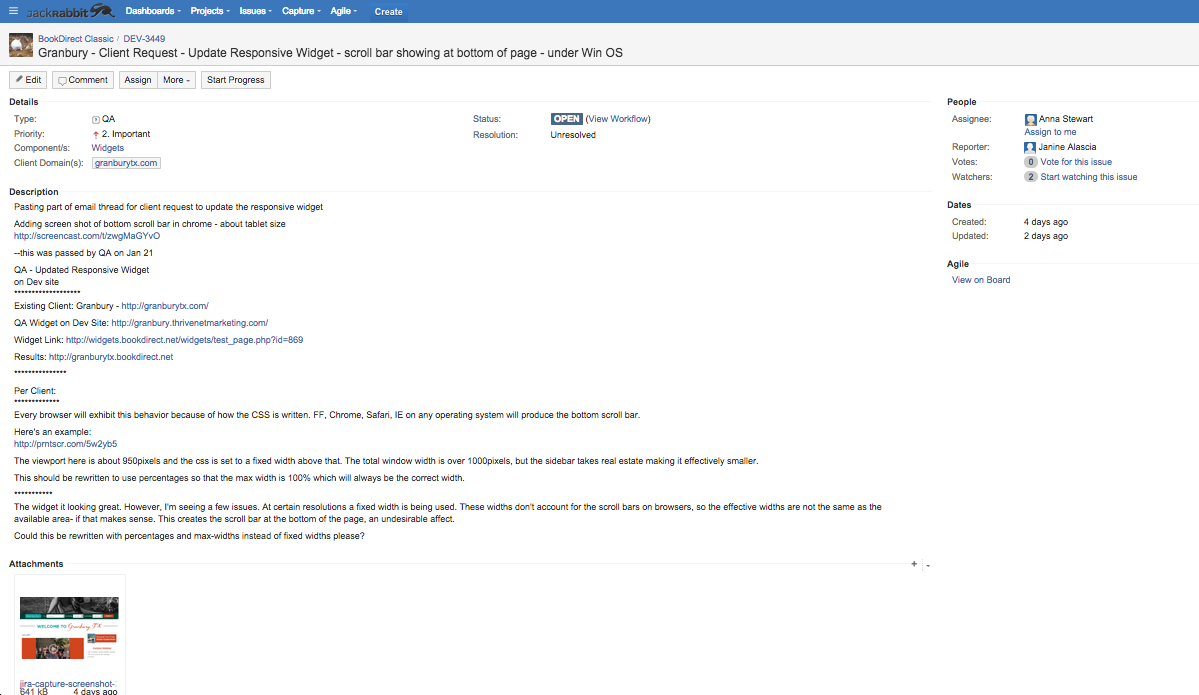
\includegraphics[bb=500 500 500 500]{issue_tracking_jira.png}
\label{fig:one}
\end{figure}

\end{document}
% End of v2-acmsmall-sample.tex (March 2012) - Gerry Murray, ACM


